\title{Linear Combinations} 
\subtitle{\SubTitleName}
\institute[]{\Course}
\author{\Instructor}
\maketitle   




\frame{\frametitle{Topics and Learning Objectives}

\Emph{Topics} \\
\TopicStatement

\begin{itemize}
    % \item  Vectors in $ \mathbb R ^{n}$, and their basic properties 
    
    \item linear combinations of vectors
    % \item the span of a set of vectors

\end{itemize}

\vspace{0.5cm}

\LO\\

\LearningObjectiveStatement

\begin{itemize}
    % \item  Apply geometric and algebraic properties of vectors in $ \mathbb R ^{n}$ to compute vector additions and scalar multiplications.
    \item  characterize a set of vectors in terms of \Emph{linear combinations}
    
\end{itemize}



}





\frame{\frametitle{Linear Combinations Definition} 

    \begin{center}\begin{tikzpicture} \node [mybox](box){\begin{minipage}{0.80\textwidth}\vspace{4pt}

        Given vectors $ \vec v_1, \vec v_2 ,\dotsc, \vec v_p \in \mathbb R ^{n} $, and scalars $ c_1 , c_2, \dotsc, c_p$,  the vector $\vec y$, where
        \begin{equation*}
        \vec y = c_1 \vec v_1 + c_2 \vec v_2 + \cdots + c_p \vec v_p
        \end{equation*}\pause 
        is called a \Emph{linear combination} of $\vec v_1, \vec v_2 ,\dotsc, \vec v_p $ with weights $ c_1 , c_2 ,\dotsc, c_p$.

    \end{minipage}};
    \node[fancytitle, right=10pt] at (box.north west) {Definition};
    \end{tikzpicture}\end{center}    
    

}





\frame{\frametitle{Linear Combinations Example} 

    Can $\vec y$ be represented as a linear combination of $\vec v_1$ and $\vec v_2$? 
    
    $$\vec y = \spalignmat{1;3}, \quad \vec v_1 = \spalignmat{1;1}, \quad \vec v_2 = \spalignmat{-1;1}$$
    \pause 
    \Emph{Solution}\\
    If $\vec y$ can be represented as a linear combination of $\vec v_1$ and $\vec v_2$, \pause we can find $c_1$ and $c_2$ so that $c_1 \vec v_1 + c_2 \vec v_2 = \vec y$. 
    \pause
    The vector equation $c_1 \vec v_1 + c_2 \vec v_2 = \vec y$ is $$ c_1\spalignmat{1;1} + c_2 \spalignmat{-1;1} = \spalignmat{1;3}$$ 
    \pause 
    Can we represent this vector equation as a system of equations? 
}





\frame{\frametitle{Linear Combinations Example}     
    Our vector equation $c_1 \vec v_1 + c_2 \vec v_2 = \vec y$ is
    $$ c_1\spalignmat{1;1} + c_2 \spalignmat{-1;1} = \spalignmat{1;3}$$ 
    \pause 
    \vspace{-2pt}
    This can be written as
    $$\spalignmat{c_1;c_1}+ \spalignmat{-c_2;c_2}= \spalignmat{c_1-c_2;c_1+c_2}= \spalignmat{1;3}$$ \pause 
    Thus, we have the linear system
    \vspace{-6pt}
    \begin{align*}
        c_1-c_2 & = 1 \\
        c_1+c_2 &= 3
    \end{align*}
    \pause There is a solution to this system, $c_1 = 2$, $c_2 = 1$. \pause Therefore, $\vec y$ can be represented as a linear combination of $\vec v_1$ and $\vec v_2$.
}





\frame{\frametitle{Linear Combinations Example}   

    We found that $2\vec v_1 + \vec v_2 = \vec y$. 
    \begin{center}
        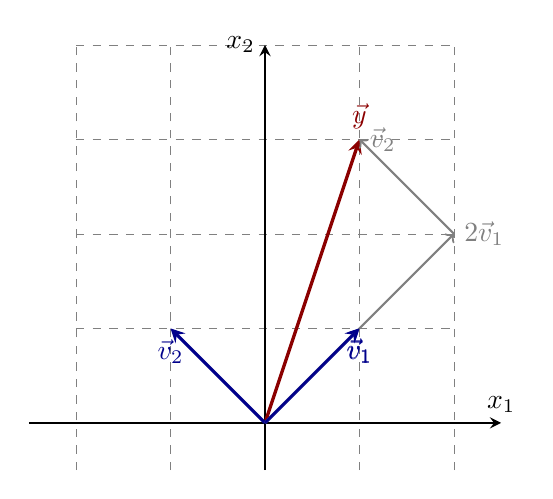
\begin{tikzpicture}[scale=1.2] 
            \onslide<2->{
            \draw[style=help lines,dashed] (-2,-0.5) grid[step=1cm] (2,4);
            \draw[->,black,thick,-stealth] (-2.5,0) -- (2.5,0) node[above] {$ x_1$}; 
            \draw[->,black,thick,-stealth] (0,-0.5) -- (0,4) node[left] {$ x_2$}; 
            }        
            \onslide<3->{
            \draw[->,DarkRed, very thick,-stealth] (0,0) -- (1,3) node[above] {$ \vec y$}; 
            \draw[->,DarkBlue, very thick,-stealth] (0,0) -- (1,1) node[below] {$ \vec v_1$}; 
            \draw[->,DarkBlue, very thick,-stealth] (0,0) -- (-1,1) node[below] {$ \vec v_2$}; 
            }
            \onslide<4->{
            \draw[->,thick,gray] (0,0) -- (2,2) node[above, right] {$ 2\vec v_1$}; 
            \draw[->,DarkBlue, thick,-stealth] (0,0) -- (1,1) node[below] {$ \vec v_1$}; 
            }    
            \onslide<5->{
            \draw[->,thick,gray] (2,2) -- (1,3) node[below, right] {$ \vec v_2$}; 
            }                
        \end{tikzpicture}
    \end{center}   

}






\frame{\frametitle{Geometric Interpretation of Linear Combinations} 

Any vector in $\R^2$ can be represented as a linear combination of two vectors in $\mathbb R^2$ that are not multiples of each other.

\vspace{6pt}
\begin{center}
   
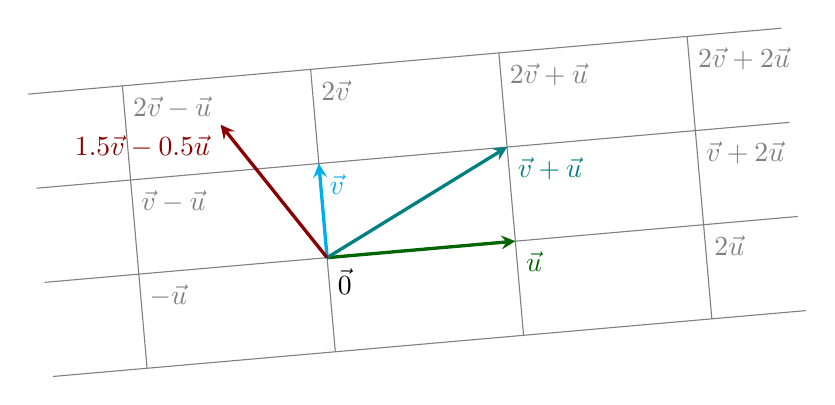
\begin{tikzpicture}[scale=1.2]
\draw[gray, thin,rotate=5]   
        (0,0)--(8,0)
        (0,1) -- (8,1)
        (0,2)--(8,2)
        (0,3)--(8,3);
\draw[gray, thin, rotate=5]
      (1,0)--(1,3)
      (3,0)--(3,3)
      (5,0)--(5,3)
      (7,0)--(7,3);
 \draw[.,Black,very thick,rotate=5] (3,1) node[anchor=north west] {$\vec 0$};
 \draw[->,DarkGreen,very thick,-stealth,rotate=5] (3,1) -- (5,1) node[anchor=north west] {$\vec u$}; 
 \draw[.,gray,very thick,rotate=5] (7,1) node[anchor=north west] {$2\vec u$};
 \draw[->,cyan,very thick,-stealth,rotate=5] (3,1) -- (3,2) node[anchor=north west] {$\vec v$}; 
  \draw[->,Teal,very thick,-stealth,rotate=5] (3,1) -- (5,2) node[anchor=north west] {$\vec v+ \vec u$};
  \draw[.,gray,very thick,rotate=5] (7,2) node[anchor=north west] {$\vec v+2\vec u$};
  \draw[.,gray,very thick,rotate=5] (7,3) node[anchor=north west] {$2\vec v+2\vec u$};
  \draw[.,gray,very thick,rotate=5] (5,3) node[anchor=north west] {$2\vec v+\vec u$};
  \draw[.,gray,very thick,rotate=5] (3,3) node[anchor=north west] {$2\vec v$};
  \draw[.,gray,very thick,rotate=5] (1,3) node[anchor=north west] {$2\vec v-\vec u$};
  \draw[.,gray,very thick,rotate=5] (1,2) node[anchor=north west] {$\vec v-\vec u$};
  \draw[.,gray,very thick,rotate=5] (1,1) node[anchor=north west] {$-\vec u$};
  \draw[->,DarkRed,very thick,-stealth,rotate=5] (3,1) -- (2,2.5) node[anchor=north east] {$1.5\vec v-0.5\vec u$};
 
 
 
 
\end{tikzpicture}   
    
\end{center}

}


\frame{\frametitle{Linear Combinations Example in $\mathbb R^3$} 

    Can $\vec y$ be represented as a linear combination of $\vec v_1$ and $\vec v_2$? 
    
    $$\vec y = \spalignmat{1;3;1}, \quad \vec v_1 = \spalignmat{1;1;0}, \quad \vec v_2 = \spalignmat{-1;1;0}$$
    \pause 
    \Emph{Solution}\\
    If $\vec y$ can be represented as a linear combination of $\vec v_1$ and $\vec v_2$, \pause we can find $c_1$ and $c_2$ so that $c_1 \vec v_1 + c_2 \vec v_2 = \vec y$. 
    \pause
    The vector equation $c_1 \vec v_1 + c_2 \vec v_2 = \vec y$ is $$ c_1\spalignmat{1;1;0} + c_2 \spalignmat{-1;1;0} = \spalignmat{1;3;1}$$ 

}


\frame{\frametitle{Linear Combinations Example in $\mathbb R^3$} 

    Expressing this as a linear system, we obtain
    \begin{align*}
        c_1-c_2 & = 1 \\
        c_1+c_2 &= 3 \\
        0c_1+0c_2 &= 1
    \end{align*}
    Thus, the system is inconsistent. 
    \begin{itemize}
        \item<2-> There is no solution to this system. 
        \item<3-> There are no values of $c_1$ and $c_2$ so that $c_1 \vec v_1 + c_2 \vec v_2 = \vec y$
        \item<4-> $\vec y$ cannot be expressed as a linear combination of the other two vectors. 
    \end{itemize}
}

\frame{\frametitle{Summary}

We explored the following concepts in this video. \vspace{4pt}
\begin{itemize}\setlength{\itemsep}{8pt}
    \item characterizing a set of vectors in terms of \Emph{linear combinations}
    \item determining whether a given vector can be represented by a linear combination of a set of vectors
\end{itemize}

}
